\documentclass[tikz,border=10pt]{standalone}
\usepackage{amsmath}
\usetikzlibrary{angles,quotes}
\begin{document}
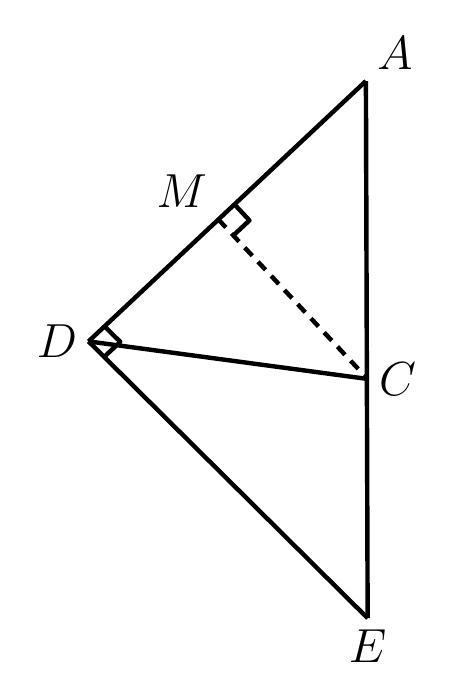
\begin{tikzpicture}[line width=1.6pt, line join=round]
\coordinate (A) at (1.776,3.433);
\coordinate (C) at (1.798,-0.351);
\coordinate (D) at (-1.747,0.126);
\coordinate (M) at (-0.099,1.676);




\coordinate (E) at (1.798,-3.389);


\draw (A) -- (E);
\draw (E) -- (D);
\draw (D) -- (A);

\draw (D) -- (C);


\draw[dash pattern=on 4pt off 3pt] (M) -- (C);


\pic[draw, angle radius=0.280cm, angle eccentricity=1.0] {right angle=A--M--C};
\pic[draw, angle radius=0.280cm, angle eccentricity=1.0] {right angle=A--D--E};


\node[above right, font=\fontsize{16}{19.2}\selectfont] at (A) {$A$};
\node[below, font=\fontsize{16}{19.2}\selectfont] at (E) {$E$};
\node[left, font=\fontsize{16}{19.2}\selectfont] at (D) {$D$};
\node[right, font=\fontsize{16}{19.2}\selectfont] at (C) {$C$};
\node[above left, font=\fontsize{16}{19.2}\selectfont] at (M) {$M$};
\end{tikzpicture}
\end{document}
